\documentclass[spanish,10pt,letterpaper,onecolumn]{article}
\usepackage[T1]{fontenc}
\usepackage[utf8]{inputenc}
\usepackage{graphicx}
\usepackage{amssymb}
\usepackage{amsthm}
\usepackage{amsmath}
\usepackage{babel}
\usepackage[left=2.50cm, right=2.50cm, top=2.50cm, bottom=2.50cm]{geometry}
\usepackage{titlesec}
\usepackage{lipsum}
\usepackage[hidelinks]{hyperref}
\usepackage{caption}
\usepackage{algorithm}
\usepackage{algpseudocode}
\usepackage{graphicx}
\usepackage{listings}
\usepackage{tikz}
\usetikzlibrary{arrows.meta, positioning, calc, decorations.markings}
\usepackage{xcolor}
\usepackage{subcaption}
\addto\captionsspanish{\renewcommand{\tablename}{Tabla}}
\captionsetup[figure]{labelfont=bf, textfont=normalfont}
\captionsetup[table]{labelfont=bf, textfont=normalfont}
\usepackage[backend=biber,style=apa]{biblatex}
\DeclareLanguageMapping{spanish}{spanish-apa}
\addbibresource{references.bib}

\begin{document}
	
	% Portada personalizada
	\begin{titlepage}
		\centering
		\vspace*{2cm}
		
		\includegraphics[width=250pt]{images/logo-uniandes.png}\par\vspace{2cm}
		
		{\Huge\bfseries Aproximación de la cinemática inversa de los brazos de un robot Pepper mediante aprendizaje por refuerzo\par}
		\vspace{2cm}
		
		{\Large \textbf{Autor}\\ Nicolás Rincón Sánchez\par}
		\vspace{0.5cm}
		{\Large \textbf{Director}\\ Fernando Enrique Lozano Martínez\par}
		\vspace{0.5cm}
		{\Large \textbf{Jurado}\\ Johann F. Osma Cruz\par}
		
		\vfill
		
		{\Large
			Universidad de los Andes\\
			Facultad de Ingeniería\\
			Departamento de Ingeniería Eléctrica y Electrónica\\
			Bogotá D.C., Colombia\\
			Julio de 2025
		}
	\end{titlepage}

	% Resumen después de página de respeto
	\newpage
	\thispagestyle{empty}
	\begin{abstract}
	Este trabajo presenta una aproximación basada en Aprendizaje por Refuerzo (RL) para resolver la cinemática inversa de los brazos de un robot Pepper. Se diseñaron dos entornos de entrenamiento empleando el framework Gymnasium para modelar los agentes correspondientes a cada brazo y un esquema de Aprendizaje Curricular que incrementa progresivamente la dificultad de los objetivos durante el entrenamiento. Posteriormente, se realizó una optimización de los hiperparámetros de dos algoritmos (PPO y SAC) para identificar cuál se desempeña mejor a la hora de generar una política adecuada para que los brazos alcancen de forma autónoma una posición específica en el espacio. Finalmente, se realizaron unas pruebas de validación con las mejores políticas obtenidas para verificar la precisión alcanzada por los brazos al llegar a poses aleatorias.
\end{abstract}

\vspace{1em}
\noindent\textbf{Palabras clave:} Aprendizaje Curricular, Aprendizaje por Refuerzo, Cinemática Inversa, Pepper

\vspace{6em}
\begin{otherlanguage}{english}
	\begin{abstract}
	This project presents an approach based on Reinforcement Learning to solve the inverse kinematics of a Pepper robot's arms. Two training environments were designed using the Gymnasium framework to model the agents for each arm, together with a Curriculum Learning scheduler that progressively increases task difficulty during training. Next, hyperparameter optimization was carried out for two algorithms (PPO and SAC) to determine which performs better at producing a policy that allows the arms to autonomously reach a given position in space. Finally, validation tests were run with the best policies obtained to verify the accuracy achieved by the arms when reaching random poses.
	\end{abstract}
	
	\vspace{1em}
	\noindent\textbf{Keywords:} Curriculum Learning, Reinforcement Learning, Inverse Kinematics, Pepper
\end{otherlanguage}
	
	\newpage
	\setcounter{page}{1} 
	
	% Tabla de contenido
	\renewcommand{\contentsname}{Tabla de contenido}
	\tableofcontents
	\newpage
	
	% Contenido
	\section{Introducción}

Pepper es un robot social desarrollado por SoftBank Robotics, diseñado para la interacción humana y ampliamente utilizado en entornos comerciales y educativos \parencite{softbank2023pepper}. Entre otras características físicas, este modelo cuenta con una base móvil y extremidades superiores con un total de 20 grados de libertad, lo que le permite realizar movimientos naturales que intentan emular la expresividad de un ser humano de la manera más natural posible \parencite{softbank2023pepper}. \\

La Facultad de Ingeniería de la Universidad de los Andes actualmente cuenta con dos ejemplares de robot Pepper, llamados Nova y Ópera, principalmente ligados a la iniciativa estudiantil SinfonIA. Estos robots han sido utilizados en diversos escenarios académicos y en eventos promocionales tanto de la iniciativa como de la universidad. Su uso en estos espacios ha demostrado el potencial de la robótica social, perfilando a la Universidad de los Andes como pionera de este campo en Colombia.\\

El éxito de estas aplicaciones ha sido posible gracias a la calibración cuidadosa de los sensores del robot y a la programación manual de su lógica de comportamiento. No obstante, estas tareas requieren una inversión considerable de tiempo y esfuerzo, ya que deben repetirse para cada situación específica. Automatizar estos procesos no solo optimizaría los tiempos de desarrollo, sino que permitiría enfocar los esfuerzos humanos en diseñar experiencias más complejas e innovadoras para la interacción.\\

Las capacidades del robot Pepper se agrupan principalmente en navegación, percepción, comunicación y manipulación. En particular, esta última se centra en el movimiento de los brazos del robot e implica operarlos como manipuladores seriales cuyo efector final es una mano capaz de señalar, agarrar, transportar y sostener objetos. Si bien el sistema operativo del robot permite controlar los ángulos articulares para alcanzar determinadas posiciones, hacerlo de forma manual exige una sintonización meticulosa y propensa a errores, lo que limita su eficiencia y escalabilidad. \\

Debido a lo anterior, se propone emplear técnicas de Aprendizaje por Refuerzo (RL, por sus siglas en inglés) para automatizar la estimación de los ángulos articulares requeridos para alcanzar una posición deseada. En este documento, se presenta un desarrollo que implementa el entrenamiento de modelos de RL a partir del ajuste de hiperparámetros de algoritmos conocidos aplicados sobre una simulación de Pepper con el fin de que aprenda, de forma autónoma, a posicionar sus brazos en coordenadas específicas.\\

La ventaja del uso de RL frente a otras aproximaciones de aprendizaje automático radica en que no se depende de una colección de datos etiquetados para el entrenamiento. Así pues, se busca que el robot aprenda a ajustar sus ángulos articulares a partir de su propia experiencia, según la recompensa o pensalización que reciba en retroalimentación por explorar diferentes configuraciones de ángulos. De este modo, Pepper puede desarrollar políticas de comportamiento que le permitan alcanzar poses precisas de forma eficiente, flexible y adaptable a distintas condiciones del entorno.\\
	
	\section{Objetivos}

\subsection{Objetivo General}

Desarrollar una aproximación basada en Aprendizaje por Refuerzo que permita al robot Pepper aprender a resolver la cinemática inversa de sus brazos para alcanzar posiciones específicas en el espacio de trabajo.

\subsection{Objetivos Específicos}

\begin{itemize}
	\item Modelar un entorno de simulación personalizado utilizando Gymnasium, que refleje de forma realista la dinámica y las restricciones cinemáticas de los brazos del robot Pepper.
	
	\item Diseñar una función de recompensa que guíe el aprendizaje del agente hacia políticas que minimicen el error entre la posición alcanzada por el efector final y una posición objetivo.
	
	\item Implementar y entrenar algoritmos de Aprendizaje por Refuerzo para optimizar las políticas del agente dentro del entorno simulado.
	
	\item Evaluar el desempeño y la capacidad de generalización de las políticas aprendidas, mediante métricas de precisión y tasa de éxito en tareas de posicionamiento.\\
\end{itemize}



	
	\section{Problemática y Justificación}

La automatización de sistemas se ha convertido en una de las ramas más importantes en la ingeniería y la industria moderna. Su propósito principal consiste en asegurar que los procesos de dicho sistema se ejecuten correctamente, toda vez que se busca reducir el tiempo que toma completarlos o la cantidad de recursos, tanto energéticos como monetarios, que se consume para realizarlos. En medio de esta optimización, los procesos deben seguir completándose y ejecutándose adecuadamente, incluso sin necesidad de supervisión e intervención humana.\\

En el campo de la robótica, la automatización es fundamental para asegurar que un robot sea capaz de completar satisfactoriamente las tareas para las cuales fue construído. Específicamente, un robot social como Pepper debe ser capaz de realizar tareas asociadas mayormente a la interacción con seres humanos. El sistema operativo del robot ofrece diversas opciones para que los desarrolladores intervengan los parámetros necesarios y permitan que el robot mueva sus brazos, hable o navegue hacia alguna ubicación especificada, para concretar su interacción con un ser humano. Así mismo, Pepper ofrece la posibilidad de recuperar los datos que obtiene de sus sensores y cámaras.\\

Actualmente, la automatización de la navegación de los robots es un problema ampliamente estudiado y que cuenta con diversas propuestas de solución enfocadas en hacer más precisos y eficientes los algoritmos de planeación de trayectoria, los cuales reciben un mapa del espacio en el que se encuentra el robot y retornan una ruta que puede seguir para llegar a un punto de destino específico. De igual manera, las tareas de percepción son estudiadas en el campo de la computación visual por medio de algoritmos de aprendizaje profundo encargados de refinar la detección de obstáculos y la decodificación y clasificación de objetos en el campo visual de una imagen, por ejemplo. Por último, las tareas de comunicación han tenido un impulso sustancial debido a la popularización de los Modelos Extensos de Lenguaje (LLMs, por sus siglas en inglés) y de igual manera, ya son estudiados y ampliamente tratados mediante técnicas de procesamiento de lenguaje natural.\\

La automatización de las tareas de manipulación o, en general, de acomodación de posiciones forma parte del problema de la cinemática inversa. Este tiene soluciones directas y ampliamente conocidas para el caso de robots simples como un robot diferencial, pero se vuelve más difícil en otro tipo de robots con geometrías más complejas. En el caso de un robot Pepper, el problema se complifica debido a que los brazos de un robot Pepper tienen cinco grados de libertad (técnicamente seis si se considera la apertura y cierre de la mano), cada uno. Al contar con un conjunto de eslabones rígidos conectados mediante articulaciones con rangos de operación limitados, un brazo del robot Pepper se puede modelar como un manipulador. \\

El problema de la cinemática inversa es complejo en un manipulador serial de dos eslabones debido a que existen múltiples soluciones para una misma posición. A medida que se incrementan los grados de libertad del manipulador, el problema aumenta de complejidad. Adicionalmente, en el caso de Pepper, otra dificultad adicional surge debido a que algunos de los eslabones del brazo de Pepper tienen dos grados de libertad asociados en lugar de solo uno. \\

A diferencia de las tareas previamente mencionadas, donde existen soluciones estandarizadas y librerías robustas, las aproximaciones tradicionales al problema de cinemática inversa se basan principalmente en métodos numéricos. Estos métodos iterativos intentan estimar ángulos articulares que lleven al efector final a la posición deseada, pero son sensibles a condiciones iniciales, pueden no converger o hacerlo a soluciones no óptimas. Igualmente, presentan limitaciones en escenarios con restricciones complejas o geometría redundante.\\

A raíz de estas limitaciones que presentan los enfoques tradicionales, el uso de técnicas de aprendizaje por refuerzo ofrece una alternativa prometedora. Este enfoque permite al robot aprender, mediante interacción continua con un entorno simulado, a ajustar los ángulos de sus articulaciones para alcanzar posiciones objetivo de manera autónoma y adaptativa. Por otro lado, al no requerir del modelado complejo de la cinemática inversa sino basarse en el aprendizaje de un comportamiento, se espera que arroje soluciones suficientemente robustas, generalizables y eficientes.\\

De esta manera, el presente proyecto surge una propuesta para encontrar una metodología algorítmica y ajustable para abordar la cinemática inversa de un manipulador complejo, como los brazos del Pepper. El planteamiento de esta aproximación contribuye, entonces, al avance de los intentos de automatización de las tareas que puede abordar un robot Pepper. Complementado con otras propuestas existentes de automatizar tareas de navegación, percepción y comunicación, busca reducir el tiempo requerido de trabajo sobre el robot para prepararlo para eventos o para apoyo en escenarios académicos, mejorando la eficiencia del proceso de desarrollo de los equipos de trabajo.\\


	
	\section{Marco Teórico}

\subsection{Aprendizaje por Refuerzo}
El aprendizaje por refuerzo, también conocido por su nombre en inglés \textit{Reinforcement Learning} (RL) es un enfoque del aprendizaje automático en el cual se busca que un agente aprenda a realizar acciones a partir de su interacción con el entorno. De manera general, todos los problemas de RL presentan tres características distintivas en común: primero, se pueden describir como problemas de lazo cerrado; segundo, el agente no conoce las acciones que debe realizar, sino que las debe descubrir por medio de exploración y dependiendo de cuáles sean las que arrojen las mejores recompensas; y tercero, las acciones que el agente toma tienen efecto sobre las acciones tomadas en un momento posterior, puesto que el agente aprende a partir de su experiencia \parencite{sutton2018reinforcement}.\\

El enfoque del aprendizaje por refuerzo se diferencia de otros paradigmas del Machine Learning como el Aprendizaje Supervisado, puesto que no se cuenta con un conjunto de entrenamiento con datos etiquetados de los cuales se pueda abstraer información para generalizar predicciones. Así mismo, se diferencia del Aprendizaje No Supervisado, puesto que el objetivo principal es que el agente aprenda de su propia experiencia a partir de los valores de una recompensa por las decisiones que toma y no que pueda abstraer patrones o estructuras sobre un conjunto existente de datos \parencite{sutton2018reinforcement}.\\

Dentro de un problema de RL se pueden caracterizar dos elementos principales. En primer lugar, un Agente que es una entidad o programa que es capaz de tomar decisiones y realizar mediciones sobre el entorno. En segundo lugar, un Entorno que comprende el contexto externo al agente cuyas condiciones pueden ser alteradas por este. El flujo lógico del RL se basa en la observación del entorno por parte del agente, específicamente del estado actual del entorno ($S_t$). Posteriormente, el agente interactúa con el entorno por medio de la realización de una acción ($A_t$). Esta acción es capaz de cambiar el estado del entorno ($S_{t+1}$), el cual le retorna al agente un valor de recompensa ($r_t$), el cual se busca maximizar por medio de la realización de las mejores acciones.\\

\begin{figure}[h!]
	\centering
	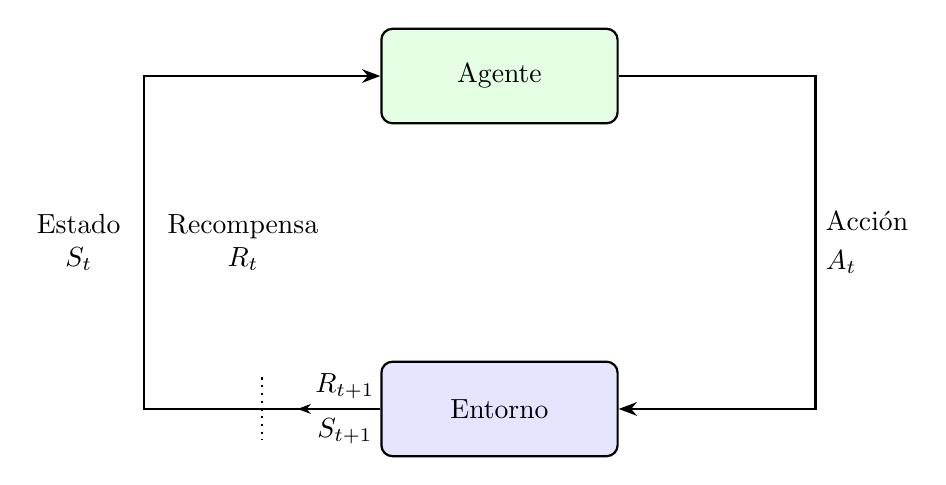
\begin{tikzpicture}[
		node distance=3cm and 4.5cm, % Distancia vertical y horizontal
		% --- Estilos ---
		caja/.style={
			draw, 
			rectangle, 
			rounded corners, 
			minimum width=3cm, 
			minimum height=1.2cm, 
			text centered, 
			thick
		},
		flecha_principal/.style={
			-Stealth, 
			thick
		},
		% Estilo para añadir una flecha en medio de un camino
		flecha_intermedia/.style={
			decoration={markings, mark=at position 0.35 with {\arrow{Stealth}}},
			postaction={decorate}
		}
		]
		% 1. Nodos: Agente arriba, Entorno abajo
		\node[caja, fill=green!10] (agent) {Agente};
		\node[caja, fill=blue!10, below=of agent] (env) {Entorno};
		
		% 2. Bucle de Acción (Derecha) - Se mantiene igual
		\draw[flecha_principal] (agent.east) -- ++(2.5,0)
		|- node[pos=0.25, right, align=left] {Acción \\[2pt] $A_t$}
		(env.east);
		
		% 3. Bucle de Retroalimentación (Izquierda) - CON FLECHA INTERMEDIA
		\draw[flecha_principal] (env.west) -- ++(-3, 0) coordinate (esquina_izq)
		|- (agent.west);
		
		% 4. Colocación de etiquetas - AHORA CENTRADAS VERTICALMENTE
		% Se crea una coordenada a medio camino vertical para usarla como referencia
		\coordinate (centro_vertical) at ($(agent.west)!0.5!(env.west)$);
		% Se colocan las etiquetas a la altura de esa coordenada
		\node[left=5pt, align=center] at (esquina_izq |- centro_vertical) {Estado \\ $S_t$};
		\node[right=5pt, align=center] at (esquina_izq |- centro_vertical) {Recompensa \\ $R_t$};
		
		% 5. Indicador de tiempo y S_{t+1}, R_{t+1} - Se mantiene igual
		\path (env.west) -- (esquina_izq) 
		node[pos=0.15, above] {$R_{t+1}$} 
		node[pos=0.15, below] {$S_{t+1}$};
		
        \path[flecha_intermedia] (env.west) -- (esquina_izq);

		% Mantenemos la línea punteada para el paso del tiempo
		\path (env.west) -- (esquina_izq) coordinate[pos=0.5] (tick_pos);
		\draw[dotted, thick] (tick_pos) ++(0, 0.4) -- ++(0, -0.8);
		
	\end{tikzpicture}
	\caption{Representación general del paradigma de aprendizaje por refuerzo.}
	\label{fig:rl-flow}
\end{figure}


El paradigma del RL se complementa con otros cuatro subelementos: 

\begin{itemize}
	\item Una política ($\pi$) que define la manera como el agente se comporta dadas las condiciones del entorno. El objetivo primordial del aprendizaje en RL es obtener buenas políticas, es decir, buenas reglas de comportamiento.
	\item Una función de recompensa que retorna un valor al agente, su recompensa ($r_t$). La función de recompensa intenta codificar la meta del entrenamiento, lo que se quiere que el agente sea capaz de aprender. El agente sólo puede recibir una recompensa, pero no puede modificarla ni interactuar con ella de otra manera que no sea sólo percibiéndola.
	\item Una función de valor que define la recompensa que el agente podría esperar recibir a largo plazo. De esta manera, la búsqueda de las mejores políticas se realiza evaluando la función de valor.
	\item Finalmente, un modelo del entorno que permita abstraer sus características principales y usarlas para estimar con la mayor precisión posible una función de valor. \parencite{sutton2018reinforcement}
\end{itemize} 

Los principales componentes, así como su interacción en un problema general de RL se pueden apreciar en la Figura \ref{fig:rl-flow}.\\


\subsubsection{Proceso de Decisión de Markov}
Un Proceso de Decisión de Markov (MDP) es un modelo matemático para la toma de decisiones secuenciales orientadas a una meta, donde cada decisión tiene un carácter probabilístico. En el aprendizaje por refuerzo, los MDP de horizonte finito son el principal objeto de estudio. Estos se pueden definir formalmente como una 5-tupla $(E, A, D_n, Q_n, r_n, g_N)$ donde $E$ es el espacio de estados, $A$ es el espacio de acciones, $D_n \subset E \times A$ es un subconjunto que contiene todos los pares estado-acción aceptables en un tiempo $n$. Se define como la relación que empareja todas las acciones que el agente puede tomar estando el entorno en un estado definido, a partir de la regla de asignación:

\begin{equation}
	D_n(x) = \{a \in A | (x,a) \in D_n\} \quad \forall x \in E
\end{equation}

$Q_n$ es una regla de transición estocástica que indica la probabilidad de que aplicar una acción $a\in A$ al encontrarse en un estado $x\in E$ en un tiempo $n$ genere un cambio a un estado $x' \in E$ en el tiempo $n+1$. Finalmente, $r_n(x,a)$ es una función que indica la recompensa que se obtendría en un paso si el sistema está en el estado $x$ y se toma la acción $a$. Por su parte, $g_N(x)$ es una función que indica la recompensa terminal en un tiempo $N$ si el estado es $x$ \parencite{bauerle2010markov}.\\

\subsubsection{Tarea de Aprendizaje en Robótica}

Es posible modelar una tarea de aprendizaje en robótica como un Proceso de Decisión de Markov individual continuo descrito por la tupla $(S,A,R,T,\gamma)$, donde $S\subset \mathbb{R}^n$ es el espacio de estados, $A\subset \mathbb{R}^m$ es el espacio de acciones, $R(s,a,s')$ es la función de recompensas que plantea el valor que se obtiene al transicionar desde un estado $s$ a otro $s'$ tomando una acción $a$, $T(s'|s,a)$ define la función de transición que determina la distribución de probabilidad de cada transición y $\gamma \in [0,1]$ es un factor de descuento que compensa la evolución en el espacio de estados de manera continua \parencite{kroemer2021review}.\\

Siguiendo el planteamiento de MDP continuo, una tarea de manipulación $M_i$ se puede formular igualmente como un caso específico de tarea de aprendizaje. En este caso, se define como una 6-tupla 

$$M_i = (S_i, A, R_i, T_i, \gamma, \tau_i)$$

que corresponde a una extensión de la definición de una tarea general como MDP. En esta metodología, se contempla el sistema interno del robot como el agente que debe aprender a realizar una tarea y se asocia el entorno y la estructura física del robot como parte del entorno. Teniendo en cuenta estas precisiones, $S_i = S_r \times S_e$ es el conjunto global de estados, denominado Espacio de Observación, que se determina como el producto cartesiano entre el conjunto de estados del robot y el conjunto de estados del entorno. $A \subset \mathbb{R}^m$ es el conjunto de acciones posibles, denominado el Espacio de Acción. $R_i(s,a,s')$ es la función de recompensa, $T_i(s'|s,a)$ es la función de transición, $\gamma$ es el factor de descuento y $\tau_i$ es un vector de números reales que codifica información relacionada con el contexto que puede complementar información del estado actual o conservar un registro histórico de las acciones tomadas \parencite{kroemer2021review}.\\

En el caso de los problemas de aprendizaje en robótica y, específicamente, en manipulación, el objetivo principal es el aprendizaje de una política de habilidad. Esto es, una política que busque la adopción de un comportamiento parametrizable para su posterior uso en un controlador intermedio entre la política y los actuadores del robot. Esto se debe a que, en tareas de manipulación, usualmente se tiene una amplia variedad de actuadores que se controlan de diversas maneras. Por ejemplo, se requiere controlar parámetros de velocidad, aceleración y torque. Si se contemplaran todos los parámetros de los actuadores para definir el Espacio de Observación y el Espacio de Acción, se complificaría el proceso de entrenamiento y la obtención de una política adecuada para alcanzar el objetivo definido \parencite{sutton2018reinforcement}.\\

Por ello, una alternativa común consiste en la representación del Espacio de Acción de forma cartesiana. De esta manera, la política de habilidad se enfoca en entrenar comportamientos que sólo busquen alcanzar objetivos definidos en un marco de referencia, usualmente centrado en el robot, evitando obtener comportamientos directamente asociados a las señales de control de los actuadores. La política se convierte en un controlador que determina valores de referencia que ingresan a otro controlador (como un PID) enfocado en el ajuste fino de la dinámica de las partes móviles del robot. Finalmente, es este controlador el encargado de ajustar las señales que ajustan los valores de las velocidades y torques de los motores que llevan al robot a alcanzar el objetivo cartesiano definido en el Espacio de Acción \parencite{kroemer2021review}.


\subsection{Aprendizaje Curricular}

En aprendizaje automático, un enfoque adoptado para mejorar la calidad del entrenamiento o acelerarlo es el del Aprendizaje Curricular. Esencialmente, se basa en la idea de realizar un ordenamiento de los datos de entrenamiento para que este suceda análogo a como aprenden los seres humanos. Es decir, partiendo de ejemplos más sencillos y específicos para diverger hacia casos más difíciles o avanzados \parencite{nekamiche2023curriculum}. Una dificultad a priori que presenta este tipo de aprendizaje es que se debe realizar la organización del currículo manualmente o empleando alguna función capaz de aprovechar una característica de interés para realizar el ordenamiento. Además, un currículo inadecuado puede dificultar el aprendizaje \parencite{weng2020curriculum}. \\

Algunas variantes ampliamente utilizadas de Aprendizaje Curricular en RL son:

\begin{enumerate}
	\item \textit{Currículo de habilidad:} Durante el proceso de entrenamiento, se abstraen habilidades que se desea que el agente aprenda. A partir de estas habilidades, se define una métrica para asignarle un nivel o grado de dificultad a las tareas relacionadas que el agente debe realizar. Siguiendo este cálculo de dificultad, se ordenan las tareas de entrenamiento en orden de dificultad ascendente. En ese orden de ideas, es una técnica útil para realizar entrenamiento de políticas enfocadas en resolución de tareas complejas o variadas en las cuales haya múltiples objetivos de aprendizaje a lograr.
	
	\item \textit{Currículo estudiante-maestro:} Se definen dos agentes complementarios. Un agente actúa como estudiante que realiza tareas durante el entrenamiento siguiendo el esquema general del RL. El estudiante le comunica a otro agente, el maestro, cuál es el resultado o valor final del entrenamiento de una tarea específica. Dependiendo del resultado, el maestro decide si modifica o no la tarea de entrenamiento.
	
	\item \textit{Currículo por Self-Play:} Se basa en la definición de dos copias del mismo agente, Alice (A) y Bob (B). El entrenamiento se basa en que A realiza un cambio sobre el entorno que lo lleva desde un estado $s_0$ hasta $s_f$. Posteriormente, A le comunica a B cuál es el estado terminal y cuál era el estado inicial y su objetivo será realizar el proceso opuesto, llevar el entorno de $s_f$ a $s_0$. Eventualmente, se definen episodios del entrenamiento en los cuales se le pide al agente B que aplique la política aprendida hasta el momento para lograr el objetivo de interés por sí mismo.
	
	\item \textit{Generación de objetivos automática:} Consiste en definir un conjunto de objetivos y asociarles un valor categórico de dificultad. Se ejecuta el entrenamiento procurando que el agente logre tener una cantidad de éxitos sobre el nivel de currículo actual. Luego, se emplean los objetivos catalogados para generar automáticamente nuevos objetivos como parte de un nuevo conjunto con un mayor valor de dificultad. A diferencia del currículo de habilidad, esta técnica es útil cuando la política esperada está enfocada en realizar sólo una tarea, pero en un amplio conjunto factible de posibles objetivos \parencite{weng2020curriculum}.
\end{enumerate}

\begin{figure}[h!]
	\centering
	
	% Primera fila
	\begin{subfigure}[b]{0.35\textwidth}
		\centering
		\includegraphics[width=0.9\textwidth]{images/marco-teorico/curr-1}
		\caption{Currículo de habilidad}
		\label{fig:curr-1}
	\end{subfigure}
	\hspace{0.05\textwidth}
	\begin{subfigure}[b]{0.35\textwidth}
		\centering
		\includegraphics[width=0.7\textwidth]{images/marco-teorico/curr-2}
		\caption{Currículo estudiante-maestro}
		\label{fig:curr-2}
	\end{subfigure}
	
	\vspace{1em}
	
	% Segunda fila
	\begin{subfigure}[b]{0.35\textwidth}
		\centering
		\includegraphics[width=0.65\textwidth]{images/marco-teorico/curr-3}
		\caption{Currículo por Self-Play}
		\label{fig:curr-3}
	\end{subfigure}
	\hspace{0.05\textwidth}
	\begin{subfigure}[b]{0.35\textwidth}
		\centering
		\includegraphics[width=0.9\textwidth]{images/marco-teorico/curr-4}
		\caption{Generación de objetivos automática}
		\label{fig:curr-4}
	\end{subfigure}
	
	\caption{Esquema ilustrativo de los tipos de currículo principales presentados por \textcite{weng2020curriculum}. Las entidades en rojo se encargan de la creación del currículo y las azules entrenan sobre la política de interés.}
	\label{fig:curriculum-types}
\end{figure}


\subsection{Proximal Policy Optimization (PPO)}

PPO es un algoritmo de la familia de gradiente de política, de tipo on-policy introducido por \textcite{schulman2017ppo}. Como otros métodos de la misma familia, PPO mantiene una política estocástica parametrizada $\pi_\theta(a|s)$ y utiliza iterativamente el algoritmo de gradiente ascendente para maximizar la recompensa esperada. La diferencia de PPO es su función objetivo con recorte (llamada Clipping Function), que permite realizar múltiples actualizaciones sobre el mismo conjunto de datos sin que la política nueva se desvíe demasiado de la anterior. En cada paso de actualización de PPO se calcula la relación de probabilidad

$$
r_t(\theta) \;=\; \frac{\pi_\theta(a_t|s_t)}{\pi_{\theta_{\text{old}}}(a_t|s_t)},
$$

y la ventaja estimada $\hat A_t$. El objetivo con recorte está dado por

$$
L^{\mathrm{CLIP}}(\theta) \;=\; \mathbb{E}_t\Big[\min\big(r_t(\theta)\,\hat A_t,\;\mathrm{clip}(r_t(\theta),1-\epsilon,1+\epsilon)\,\hat A_t\big)\Big],
$$

donde $\epsilon>0$ es un parámetro pequeño. Esta formulación recompensa el cambio de política que aumenta la probabilidad de acciones con ventaja positiva, pero impone un límite fijo $(1\pm \epsilon)$ a la relación de probabilidad para evitar grandes saltos de política \parencite{schulman2017ppo}.\\

El algoritmo se puede describir mediante el siguiente pseudocódigo \parencite{schulman2017ppo}:

\begin{algorithm}
	\caption{Proximal Policy Optimization (PPO)}\label{alg:ppo}
	\begin{algorithmic}[1]
		\For {$\text{iteración}=1,2,...$}
		\For {$\text{actor}=1,2,...,N$}
		\State $\text{Ejecutar la política } \pi_{\theta_\text{old}} \text{ en el entorno durante } T \text{ timesteps}$
		\State $\text{Calcular los estimadores de ventaja } \hat{A}_1, ..., \hat{A}_{T}$
		\EndFor
		\State $\text{Optimizar el surrogado } L \text{ respecto a } \theta \text{, con } K \text{ épocas y tamaño de MiniBatch } M \leq NT$
		\State $\theta_{old} \leftarrow \theta$
		\EndFor
	\end{algorithmic}
\end{algorithm}


\subsection{Soft Actor-Critic (SAC)}

Soft Actor-Critic es un algoritmo off-policy de tipo actor-crítico desarrollado por \textcite{haarnoja2018sac}. SAC emplea una política estocástica continua $\pi_\theta(a|s)$ y dos funciones de valor $Q_{\phi_1}(s,a)$ y $Q_{\phi_2}(s,a)$ para mayor estabilidad. Su característica principal es incorporar un término de entropía máxima. El actor maximiza tanto la recompensa esperada como la entropía de la política, lo cual favorece la exploración continua \parencite{haarnoja2018sac}. En la práctica, la política se entrena para maximizar el objetivo. Equivalente a esto, en cada paso de actualización se realiza descenso de gradiente para maximizar el valor esperado de este. \\

Por otro lado, las redes $Q_{\phi_i}$ se actualizan mediante regresión TD utilizando el objetivo de Bellman suavizado por entropía. y se minimiza el error cuadrático de la función Q en ambas redes \parencite{haarnoja2018sac}. A esta técnica de suavizado en los pasos de actualización se le denomina soft updates y son lo que da nombre al algoritmo. En resumen, SAC combina aprendizaje off-policy con un término de entropía en el actor y el critico, logrando actualizaciones estables y eficiente exploración \parencite{haarnoja2018sac}. \\

El algoritmo se puede describir mediante el siguiente pseudocódigo \parencite{haarnoja2018sac}:

\begin{algorithm}
	\caption{Soft Actor-Critic (SAC)}\label{alg:sac}
	\begin{algorithmic}[1]
		\State $\text{Inicializar vectores de parámetros } \psi, \bar{\psi}, \theta, \phi$
		\For {cada iteración}
		\For {cada paso del entorno}
		\State $\mathbf{a}_t \sim \pi_\phi (\mathbf{a}_t|\mathbf{s}_t)$
		\State $\mathbf{s}_{t+1} \sim p(\mathbf{s}_{t+1}|\mathbf{s}_t,\mathbf{a}_t)$
		\State $\mathcal{D} \leftarrow \mathcal{D} \cup \{\mathbf{s}_t,\mathbf{a}_t,r(\mathbf{s}_t,\mathbf{a}_t),\mathbf{s}_{t+1}\}$
		\EndFor
		\For {cada paso del gradiente}
		\State $\psi \leftarrow \psi - \lambda_V \hat{\nabla}_\psi J_V(\psi)$
		\State $\theta_i \leftarrow \theta_i - \lambda_Q \hat{\nabla}_{\theta_i} J_Q(\theta_i) \text{ para } i\in{1,2}$
		\State $\phi \leftarrow \phi - \lambda_\pi \hat{\nabla}_\phi J_\pi(\phi)$
		\State $\bar{\psi} \leftarrow \tau\psi + (1-\tau)\bar{\psi}$
		\EndFor
		\EndFor
	\end{algorithmic}
\end{algorithm}


\subsection{Problema de Cinemática Inversa en Robótica}

La cinemática inversa (IK) es el problema de calcular las posiciones articulares de un manipulador que permiten al efector final alcanzar una orientación y posición deseadas en el espacio. En otras palabras, dada una meta $\mathbf{x}^*$ para el efector final, se busca el vector de ángulos articulares $\mathbf{q}$ tal que $f(\mathbf{q})=\mathbf{x}^*$, donde $f$ es la función cinemática directa. Este problema suele ser no lineal y multivariable \parencite{elhussieny2017inverse}. \\

A nivel matemático, es posible plantear el problema de IK general tomando como base los principios geométricos de la cinemática directa, la cual estudia la determinación de posiciones cartesianas partiendo de los valores de los ángulos articulares conocidos. Esto se logra por medio de la definición de matrices de transformación de coordenadas cartesianas:

$$H = \begin{bmatrix}
	R_n^0 & o_n^0 \\
	\mathbf{0} & 1
	\end{bmatrix}
$$

donde $R_n^0$ es una matriz de rotación acumulada a lo largo de los ejes cartesianos y $o_n^0$ es una matriz de traslación espacial. Se agrega una cuarta columna para mantener la consistencia dimensional y la escala en caso de ser necesaria, pero por defecto es unitaria. Así pues, el problema de IK es equivalente matemáticamente a encontrar una solución del vector $(q_1, q_2, ..., q_n)$ que satisfaga la ecuación:

\begin{equation}
	T_n^0(q_1, q_2, ..., q_n) = A_1(q_1) A_2(q_2) ... A_n(q_n) = H
\end{equation}

Adicionalmente, cabe resaltar que los manipuladores redundantes (aquellos que tienen más de 6 DOF) pueden tener infinitas soluciones, mientras que en posiciones singulares como articulaciones alineadas la solución puede no existir o ser inestable \parencite{elhussieny2017inverse}. Robots complejos como Pepper ejemplifican esta dificultad pues cuenta con una base omnidireccional de 3 DOF, torso con 3 DOF, cabeza 2 DOF y cada brazo 5 DOF (más dedos), sumando alrededor de 18 DOF totales \parencite{softbank2023pepper}. La alta redundancia de Pepper implica infinitas configuraciones articulares para una misma posición del efector, y además la cinemática no admite una solución analítica sencilla en general.\\

\subsubsection{Métodos clásicos de solución de IK}

Los métodos clásicos para resolver cinemática inversa suelen basarse en aproximaciones numéricas del jacobiano o soluciones analíticas parciales. Entre ellos destacan: 

\begin{itemize}
	\item \textbf{Método del jacobiano inverso}: ajusta iterativamente los ángulos articulares usando la pseudoinversa del jacobiano para acercar el efector a la posición deseada.
	
	\item \textbf{Método del jacobiano transpuesto o de gradiente}: emplea la transpuesta del jacobiano como dirección de corrección, similar a un descenso de gradiente clásico.
	
	\item \textbf{Métodos de mínimos cuadrados amortiguados}: introduce un término de regularización para mejorar la estabilidad en configuraciones cercanas a singularidades \parencite{zhao2024inverse}.
\end{itemize}


También se encuentran soluciones analíticas geométricas en robots especiales (métodos algebraicos basados en transformaciones de coordenadas), pero son poco generales. En la práctica, estas técnicas requieren cuidadosa sintonización de parámetros como pasos de actualización o criterios de convergencia, y pueden tener dificultades cerca de singularidades o límites articulares.\\

\subsubsection{Métodos basados en RL para solución de IK}

En contraste, los enfoques de aprendizaje automático y reforzado evitan formular explícitamente la cinemática y aprenden directamente políticas o modelos para alcanzar la meta. Por ejemplo, existen propuestas de algoritmos como MAPPO-IK, el cual está basado en PPO, para un manipulador de 6 DOF. En este escenario, el diseño del agente RL fue elaborado para recibir la diferencia de posición esperada-calculada como recompensa de cada paso \parencite{zhao2024inverse}. De manera similar, se ha propuesto el entrenamiento de un agente sobre un simulador de robot humanoide para resolver la cinemática inversa mediante una política similar, pero de carácter estocástico a la hora de definir la recompensa \parencite{adjei2024safe}.\\ 

De igual manera, se han planteado desarrollos que emplean redes neuronales profundas (Aprendizaje por Refuerzo Profundo) para aprender la relación inversa de un manipulador sin necesidad de calcular explícitamente las matrices jacobianas \parencite{liu2021deep}. En general, estas soluciones basadas en RL pueden adaptarse mejor a entornos dinámicos o restricciones complejas (posturas factibles, colisiones), aunque suelen requerir entrenamiento previo intensivo. Además del RL directo para IK, la literatura reciente destaca dos aproximaciones distintas. En particular, conviene mencionar trabajos que combinan aprendizaje reforzado con restricciones de seguridad y razonamiento de recompensas para garantizar trayectorias seguras en brazos robóticos \parencite{ozalp2024advancements}. \\

Por último, en la misma línea de los algoritmos propios del RL, se han desarrollado enfoques basados en Deep Q-Networks (DQN) para resolver la cinemática inversa de un manipulador de 7 DOF, usando la formulación de Producto de Exponenciales (PoE) para la cinemática directa y generando trayectorias articulares discretas con alta estabilidad frente a la sensibilidad de hiperparámetros típica de métodos continuos \parencite{malik2022deeprl}. Estos trabajos ilustran cómo tanto la revisión estructurada del estado del arte como la aplicación práctica de RL pueden avanzar la resolución de IK en manipuladores complejos.\\

	
	\section{Metodología}

\subsection{Diseño de la representación del problema}

Teniendo en cuenta la definición de una tarea de aprendizaje en robótica, se planteó el modelo del sistema siguiendo la representación propia del RL. En este orden de ideas, se definieron dos agentes independientes entre sí que corresponden al brazo derecho y el brazo izquierdo del robot. Se establece el entorno como el conjunto de articulaciones de los brazos del robot, junto con el resto de la estructura física externa a los dos brazos, ubicadas en el espacio tridimensional con la base del robot centrada en el origen $(0,0,0)$.\\

Siguiendo lo establecido por \textcite{kroemer2021review}, se plantea el problema como una Tarea de Manipulación mediante el enfoque de un Proceso de Decisión de Markov. Así pues, se emplea el enfoque de la definición de un Espacio de Observación tabular y un Espacio de Acción de tipo cartesiano. A continuación, se detallan los elementos fundamentales del planteamiento del problema como un problema de RL:

\begin{enumerate}
	\item \textbf{Espacio de Observación: } En el espacio de observación se definen los estados posibles que puede tener el entorno en cualquier momento de ejecución. En vista de que la cinemática inversa busca determinar los valores de los ángulos articulares, estas mediciones deben formar parte del espacio. 
	
		\begin{table}[h!]
		\centering
		\caption{Descripción de las variables del espacio de observación ($S$)}
		\begin{tabular}{|c|c|}
			\hline
			\textbf{Variable} & \textbf{Descripción} \\
			\hline
			$\theta_1$ & Valor del ángulo en radianes para la articulación \textit{ShoulderPitch} \\
			\hline
			$\theta_2$ & Valor del ángulo en radianes para la articulación \textit{ShoulderRoll} \\
			\hline
			$\theta_3$ & Valor del ángulo en radianes para la articulación \textit{ElbowYaw} \\
			\hline
			$\theta_4$ & Valor del ángulo en radianes para la articulación \textit{ElbowRoll} \\
			\hline
			$\theta_5$ & Valor del ángulo en radianes para la articulación \textit{WristYaw} \\
			\hline
			$e_x$ & Distancia entre posiciones $x_{actual}$ y $x_{goal}$ \\
			\hline
			$e_y$ & Distancia entre posiciones $y_{actual}$ y $y_{goal}$ \\
			\hline
			$e_z$ & Distancia entre posiciones $z_{actual}$ y $z_{goal}$ \\
			\hline
		\end{tabular}
		\label{tab:obs_var}
	\end{table}
	
	Así mismo, por practicidad a la hora de realizar el entrenamiento y para evitar sesgar al agente para que tome una ruta en particular o la priorice sobre otra, se recurre a integrar el valor del error en las tres direcciones cartesianas rectangulares con el objetivo de poder realizar una medición de la distancia entre la posición en la que se encuentra el efector final en un momento dado y la posición esperada, para así realizar un ajuste o determinar la ocurrencia de un éxito. La estructura del espacio de observación se muestra en la Tabla \ref{tab:obs_var} y los rangos de cada variable a continuación:
	
	\begin{table}[h!]
		\centering
		\caption{Rangos de valores para cada variable por brazo}
		\begin{tabular}{|c|c|c|}
			\hline
			\textbf{Variable} & \textbf{Rango (Izquierdo)} & \textbf{Rango (Derecho)} \\
			\hline
			$\theta_1$ & $[-2.0857, 2.0857] \text{ rad}$ & $[-2.0857, 2.0857] \text{ rad}$ \\
			\hline
			$\theta_2$ & $[0.0087, 1.5620] \text{ rad}$ & $[-1.5620, -0.0087] \text{ rad}$ \\
			\hline
			$\theta_3$ & $[-2.0857, 2.0857] \text{ rad}$ & $[-2.0857, 2.0857] \text{ rad}$ \\
			\hline
			$\theta_4$ & $[-1.3614, -0.0087] \text{ rad}$ & $[0.0087, 1.3614] \text{ rad}$ \\
			\hline
			$\theta_5$ & $[-1.8239, 1.8239] \text{ rad}$ & $[-1.8239, 1.8239] \text{ rad}$ \\
			\hline
			$e_x$ & $[-\infty, +\infty] \text{ m}$ & $[-\infty, +\infty] \text{ m}$ \\
			\hline
			$e_y$ & $[-\infty, +\infty] \text{ m}$ & $[-\infty, +\infty] \text{ m}$ \\
			\hline
			$e_z$ & $[-\infty, +\infty] \text{ m}$ & $[-\infty, +\infty] \text{ m}$ \\
			\hline
		\end{tabular}
		\label{tab:obs_rangos}
	\end{table}
	
	
	\item \textbf{Espacio de Acción: } En el espacio de acción se definen las posibles acciones que toman los agentes. De esta manera, como el objetivo principal consiste en alterar los valores de los ángulos en cada ejecución, se codifica los cambios que se le deben aplicar a cada ángulo en un paso. El agente tiene la potestad de decidir si aplica una o varias acciones en un paso específico. Los valores establecidos como límites máximo y mínimo buscan asegurar que el movimiento en cada paso sea suave y así reducir un posible daño en el robot e incluso permitiendo tiempo de reacción de emergencia en caso de ser necesario. La estructura del espacio de acción es la siguiente:
	
	\begin{table}[h!]
		\centering
		\caption{Descripción del espacio de acción ($A$) para cualquier brazo}
		\begin{tabular}{|c|c|}
			\hline
			\textbf{Acción} & \textbf{Rango} \\
			\hline
			$\Delta\theta_1$ & $[-0.50, 0.50] \text{ rad}$ \\
			\hline
			$\Delta\theta_2$ & $[-0.50, 0.50] \text{ rad}$ \\
			\hline
			$\Delta\theta_3$ & $[-0.50, 0.50] \text{ rad}$ \\
			\hline
			$\Delta\theta_4$ & $[-0.50, 0.50] \text{ rad}$ \\
			\hline
			$\Delta\theta_5$ & $[-0.50, 0.50] \text{ rad}$ \\
			\hline
		\end{tabular}
		\label{tab:accion_space}
	\end{table}
	
	\item \textbf{Función de Recompensa: } La función de recompensa se diseña para establecer las aportaciones y penalizaciones compuestas que debe recibir el agente en cada paso del entrenamiento para evaluar la correctitud de la política vigente que se está explotando en ese momento. La función se diseñó a partir de ajustes experimentales buscando favorecer determinados comportamientos sobre otros, particularmente, el acercamiento al punto objetivo por parte del efector final y la ocurrencia de un éxito, definido este como un error menor a 2cm. Matemáticamente, se puede expresar de la siguiente manera:
	
	\begin{equation}
		r_n(s) = \sum_{k} R_n^{k}
	\end{equation}
	
	donde corresponde a la sumatoria de un conjunto de funciones parciales que calculan penalizaciones y contribuciones según los criterios:
	\begin{itemize}
		\item Mejoramiento del error respecto al paso inmediatamente anterior. Es decir, si el efector final se ha acercado más a la posición esperada.
		
		\begin{equation}
			R_{n}^{\text{improvement}} = 30 \cdot (d_{n-1} - d_{n})
		\end{equation}
		
		\item Penalización constante dependiendo del error (medido como la distancia euclidiana entre la posición del efector final y la posición deseada) calculado a partir de las mediciones de los errores unidimensionales en el espacio de observación como $d_n = \sqrt{e_x^2 + e_y^2 + e_z^2}$.
		
		\begin{equation}
			R_{n}^{\text{proximity}} = -2.0 \cdot d_n
		\end{equation}
		
		\item Suavidad de los movimientos del brazo, penalizado de forma constante dependiendo de qué tan extremos son las variaciones de los ángulos articulares en la contribución total de las acciones por cada paso.
		
		\begin{equation}
			R_{n}^{\text{smoothness}} = -0.15 \cdot \left|\Delta\theta\right|^2
		\end{equation}
		
		\item Penalización por alcanzar los límites de alguno de los ángulos articulares con una tolerancia de $\pm 1.0\times10^{-6}$, en cuyo caso se le quita a la recompensa total. Este término surge de la necesidad de proteger la operatividad del robot y evitar que alcance ángulos por fuera de lo permitido por la configuración del hardware y los mecanismos que permiten el movimiento adecuado del brazo. 
		
		\begin{equation}
			R_{n}^{\text{limit}} =
			\begin{cases}
				-0.75 & \text{si } \theta_i = \theta_{i,\min} \lor \theta_i = \theta_{i,\max} \quad \forall i \in \{1,2,3,4,5\} \\
				0 & \text{de lo contrario}
			\end{cases}
		\end{equation}
		
		\item Finalmente, una recompensa especial por alcanzar una posición final con un error menor a 2cm, el cual fue definido como el valor del umbral del éxito durante entrenamiento. Esta recompensa busca asegurar que el agente no pierda de vista el objetivo primordial que es alcanzar la posición final deseada. Se estableció el valor de 2cm puesto que en la práctica corresponde a una diferencia poco significativa que permitiría, en la mayoría de casos, aprovechar la configuración alcanzada para realizar alguna tarea local como agarrar un objeto, por ejemplo.
		
		\begin{equation}
			R_{n}^{\text{success}} =
			\begin{cases}
				25.0 & \text{si } d_n \leq 0.02 \\
				0 & \text{de lo contrario}
			\end{cases}
		\end{equation}
		
	\end{itemize}
	
	\item \textbf{Currículo: } El planteamiento del método de currículo se realizó a partir de las técnicas expuestas por \textcite{weng2020curriculum}. Se decidió emplear la técnica de Generación Automática de Objetivos y como estrategia para realizar el agrupamiento de los objetivos definidos por nivel de dificultad, se utilizó una medida que se optó por denominar como \textbf{Radio de Currículo}.\\
	
	El radio de currículo define una zona esférica alrededor del objetivo dentro de la cual se inicializa la posición del efector final al comienzo de cada episodio de entrenamiento. Al inicio, el radio es pequeño arrancando con un valor de 10cm, lo que implica que el robot comienza cerca del objetivo. Así se facilita el aprendizaje de movimientos básicos al inicio del entrenamiento. A medida que el agente mejora su desempeño, el radio se incrementa gradualmente, presentando desafíos más complejos al alejar la posición inicial del objetivo. Esta técnica permite que el robot construya sus habilidades de forma escalonada, promoviendo una convergencia más estable y eficiente hacia políticas de control más generalizadas.\\
	
	En este diseño, el radio del currículo inicia con un valor de 0.00 y automáticamente incrementa de a 10cm una vez que se hayan alcanzado 5 intentos exitosos consecutivos con un mismo radio. El tener 5 éxitos consecutivos asegura que la política aprendida hasta entonces ha logrado superar adecuadamente el desafío de alcanzar las poses finales para el nivel de dificultad propuesto hasta entonces. El valor del radio del currículo $c$ por cada nivel $k$ viene dado por:
	
	$$
		c_k = \min(c_{k-1}+\Delta c, c_{\max})
	$$
	
	donde se reitera que $\Delta c = 0.1$ y $c_{\max} = 0.51$, ambas expresadas en metros, que corresponde a la media de distancia entre todos los puntos factibles alcanzables en los espacios de trabajo de ambos brazos, los cuales se mostrarán en simulación más adelante.
	
\end{enumerate}


\subsection{Entrenamiento con sintonización de hiperparámetros}

Una vez definido el modelo del problema, con la definición de los agentes, los espacios de observación y acción, la función de recompensa y la técnica de incremento curricular, el siguiente paso a seguir consiste en establecer la forma de entrenar. Se planteó el uso de dos algoritmos diferentes, PPO y SAC, para realizar una comparación entre el resultado de ambos. Esta decisión se tomó por dos motivos: en primer lugar, la oportunidad de comparar el desempeño entre un algoritmo basado en política como PPO y un algoritmo basado en valor como SAC para ver cuál enfoque resulta mejor en el problema en cuestión. El montaje del entorno aprovechó el ambiente orientado al RL Gymnasium introducido por \textcite{towers2024gymnasium}, que permite programar entornos personalizados acorde al planteamiento conceptual de los mismos.\\

En segundo lugar, los dos algoritmos seleccionados tienen una implementación existente de código abierto realizada por \textcite{raffin2021stable} como parte del framework Stable Baselines 3, el cual está diseñado específicamente para facilitar la programación de tareas relacionadas con RL. Stable Baselines tiene incorporados métodos orientados al entrenamiento, aleatorización de muestras, guardado de políticas y carga de las mismas en formatos de archivo compatibles con su sistema de codificación interno y también con el ambiente de Gymnasium así como sus definiciones de entornos personalizados \parencite{raffin2021stable}.\\

Como la implementación de los algoritmos mencionados en Stable Baselines 3 tiene una serie de hiperparámetros ajustables que pueden cambiar sustancialmente los resultados de entrenamiento de una política, se acudió al framework de optimización de hiperparámetros Optuna presentado por \textcite{optuna_2019}. Optuna es capaz de realizar estudios de optimización sobre un espacio de hiperparámetros especificados junto con su rango discreto y/o categórico de valores posibles. Optuna se encarga de seleccionar valores factibles dentro del rango especificado y configurar instancias de los algoritmos con dichos hiperparámetros. Finalmente, la herramienta emplea la maximización de la recompensa notificada por el entorno para seleccionar el mejor de los estudios asociado a la mejor combinación de hiperparámetros y, por ende, la mejor política aprendida.\\

Para el caso de los algoritmos PPO y SAC, se establecieron las siguientes referencias para configurar los estudios de Optuna y realizar \textit{trials} de entrenamiento de manera secuencial:

\begin{table}[h!]
	\centering
	\caption{Espacio de hiperparámetros explorado para PPO}
	\begin{tabular}{|l|c|l|}
		\hline
		\textbf{Hiperparámetro} & \textbf{Tipo} & \textbf{Rango de valores} \\
		\hline
		\texttt{learning\_rate} & Float & $[1\times10^{-5}, 1\times10^{-3}]$ \\
		\texttt{n\_steps} & Categórico & \{256, 512, 1024, 2048\} \\
		\texttt{gamma} & Float & $[0.9, 0.9999]$ \\
		\texttt{gae\_lambda} & Float & $[0.8, 0.99]$ \\
		\texttt{ent\_coef} & Float & $[1\times10^{-8}, 1\times10^{-1}]$ \\
		\texttt{clip\_range} & Float & $[0.1, 0.4]$ \\
		\texttt{vf\_coef} & Float & $[0.1, 1.0]$ \\
		\texttt{batch\_size} & Categórico & \{64, 128, 256\} \\
		\hline
	\end{tabular}
	\label{tab:optuna-ppo}
\end{table}

\begin{table}[h!]
	\centering
	\caption{Espacio de hiperparámetros explorado para SAC}
	\begin{tabular}{|l|c|l|}
		\hline
		\textbf{Hiperparámetro} & \textbf{Tipo} & \textbf{Rango de valores} \\
		\hline
		\texttt{learning\_rate} & Float & $[1\times10^{-5}, 1\times10^{-3}]$ \\
		\texttt{buffer\_size} & Categórico & \{100000, 300000, 1000000\} \\
		\texttt{batch\_size} & Categórico & \{128, 256, 512\} \\
		\texttt{tau} & Float & $[0.005, 0.05]$ \\
		\texttt{gamma} & Float & $[0.9, 0.9999]$ \\
		\texttt{train\_freq} & Categórico & \{1, 4, 8, 16\} \\
		\texttt{gradient\_steps} & Categórico & \{-1, 1, 4, 8, 16\} \\
		\texttt{ent\_coef} & Fijo & 'auto' \\
		\hline
	\end{tabular}
	\label{tab:optuna-sac}
\end{table}

Finalmente, para ejecutar los estudios de Optuna de manera eficiente, se utilizó la táctica del Entrenamiento sobre Modelo Surrogado. Básicamente, esta consiste en crear una copia del entorno con menos restricciones o menor especificidad para que los episodios de entrenamiento se puedan ejecutar con mayor velocidad. Esta táctica permite ahorrar tiempo de entrenamiento y permitir el completamiento de una mayor cantidad de \textit{trials} de Optuna en la ventana de timeout, la cual se estableció en 8 horas para cada agente.\\

En este caso, la simplificación del entorno consistió en suprimir el modelo del agente sobre el mundo simulado. Así, el modelo surrogado consistió en una copia netamente matemáticamente del modelo completo, sobre la cual no se consideran los efectos de la física del robot sino solamente las mediciones observables en el espacio de observación y los cálculos de posicionamiento realizables con estos valores para determinar los errores, e igualmente compatible con Gymnasium \parencite{towers2024gymnasium}. La ventaja de esta táctica es que, sin pérdida de generalidad, la política aprendida tiene exactamente el mismo comportamiento, pero vinculado a tiempo del computador en lugar del tiempo simulado del movimiento del robot físico. En este proyecto, cada entrenamiento se realizó sobre 1.000.000 de timesteps. \\

\subsection{Visualización mediante simulación}

Para visualizar el comportamiento del robot y de los brazos entrenados se acudió a un simulador de código abierto qiBullet desarrollado por \textcite{busy2019qibullet}. La utilidad de qiBullet se refleja en que permite simular fielmente la física del entorno como el valor de la gravedad, torque, control de motores y velocidades de movimiento de los componentes de los robots de Softbank Robotics, teniendo modelos URDF de Pepper, Nao y Romeo. En el caso de este proyecto, se empleó el modelo URDF de Pepper. Por otro lado, aprovechando la flexiblidad de Gymnasium, se construyeron entornos compatibles con qiBullet \parencite{towers2024gymnasium}.\\

El proceso de instalación y configuración de qiBullet se encuentra disponible en la Wiki del repositorio oficial \footnote{\url{https://github.com/softbankrobotics-research/qibullet/wiki}}. Una vez instalado, existen archivos de prueba que pueden resultar útiles para verificar el correcto funcionamiento de la simulación y para familiarizarse con la orientación del robot materializado en el entorno básico e incluso probar interacción manualmente con el mouse. \\

\begin{figure}[h!]
	\centering
	\includegraphics[width=350pt]{images/metodologia/qibullet}
	\caption{Ejecución local del simulador qiBullet con un modelo del robot Pepper}
	\label{fig:qibullet}
\end{figure}

El simulador de qiBullet fue utilizado, además, para generar una visualización del espacio de trabajo de los brazos del robot. Para generar el espacio de trabajo del robot, se recurrió al método de muestreo aleatorio basado en puntos. De esta manera, considerando los rangos útiles de las articulaciones del robot presentados en la Tabla \ref{tab:obs_rangos}, se realizan selecciones aleatorias y se utilizan las ecuaciones de cinemática directa para calcular la posición del efector final y mapearla sobre la simulación para mejorar la apreciación del espacio alcanzable por cada brazo.\\

En total, se realiza un muestreo de 8 repeticiones, lo cual resulta en $8^5 = 32065$ configuraciones posibles que se mapean por cada brazo. Estos puntos finales son conservados en una estructura de datos en memoria para poder acceder a ella durante el entrenamiento y durante las pruebas. Los puntos objetivo para un radio de currículo específico se seleccionan desde este conjunto de puntos alcanzables, así como los puntos para realización de pruebas con las mejores políticas.\\

Cabe resaltar que, en simulación, la posición del efector final medida se ubica en lo que corresponde al inicio de la muñeca del brazo. Técnicamente, es el extremo inicial del efector final en lugar del extremo final. Sin embargo, para simplificar el modelo se prefirió utilizar esta coordenada para realizar los cálculos de error sin contemplar el offset relacionado a la longitud de la mano de 6.950 cm (sobre el eje x de su sistema local de referencia) de acuerdo con la documentación oficial del robot \parencite{softbank2023pepper}. \\

\begin{figure}[h!]
	\centering
	\includegraphics[width=200pt]{images/metodologia/workspace}
	\caption{Visualización del espacio de trabajo alcanzable de cada brazo superpuesto a la simulación. Los puntos en azul muestran el espacio de trabajo del brazo izquierdo y los rojos el del brazo derecho.}
	\label{fig:workspace}
\end{figure}

Esta ubicación de la coordenada de medición se puede apreciar en la Figura \ref{fig:workspace}, donde se el ángulo en el cual está orientada la visualización deja ver que los puntos que muestrean la pose estándar con todos los ángulos en cero, se encuentran sobre las muñecas en ambos brazos.


\subsection{Ejecución de pruebas de funcionamiento}

La ejecución de las pruebas de funcionamiento se realizó siguiendo el protocolo descrito a continuación:

\begin{enumerate}
	\item Generar un archivo de caché donde se almacenan los puntos muestreados del espacio de trabajo factible. Si el archivo ya existe, aprovecharlo y cargar los puntos en memoria.
	
	\item Seleccionar aleatoriamente 1000 puntos del espacio de trabajo.
	
	\item Iniciar un episodio de máximo 250 timesteps con el robot posicionado en una pose aleatoria diferente a la pose de destino, a partir de los métodos de Gymnasium.
	
	\item Reproducir la política en proceso de prueba con el agente entrenado (brazo izquierdo o brazo derecho) hasta que se alcance una posición final ubicada a una distancia menor que el umbral de precisión configurado.
	
	\item La ejecución de la prueba calcula la media y el error de precisión de la distancia entre la posición del efector final y la posición deseada. Además, retorna un conteo de la cantidad de episodios exitosos dentro de las pruebas realizadas.
\end{enumerate}

Nuevamente, para agilizar el proceso de pruebas se diseñó un argumento de ejecución que permite realizar el lanzamiento de la ráfaga de pruebas con interfaz gráfica (mostrando el movimiento en el simulador) o en consola (mostrando simplemente el resultado de cada prueba y la cantidad de episodios necesarios para llegar a la posición considerada como éxito).\\

En la Figura \ref{fig:test-gui} se muestra cómo se visualiza una prueba con interfaz gráfica. El robot inicia en una posición diferente a la de destino y realiza un movimiento de sus articulaciones permaneciendo estático en las demás articulaciones (base, torso y cabeza) hasta llegar a la posición esperada, indicada con un punto, como se ve en la Figura \ref{fig:test-start}. Una vez que llega a la posición deseada dentro del margen de precisión esperado, el punto desaparece y permite ver la pose final del robot para lograr el objetivo, como se aprecia en la Figura \ref{fig:test-reached}. De lo contrario, si no es exitosa, automáticamente se reinicia el entorno de Gymnasium e inicia la siguiente prueba.

\begin{figure}[h!]
	\centering
	
	\begin{subfigure}[b]{0.45\textwidth}
		\centering
		\includegraphics[width=\textwidth]{images/metodologia/test_start}
		\caption{Estado inicial de una prueba}
		\label{fig:test-start}
	\end{subfigure}
	\hfill
	\begin{subfigure}[b]{0.465\textwidth}
		\centering
		\includegraphics[width=\textwidth]{images/metodologia/test_reached}
		\caption{Estado exitoso de una prueba}
		\label{fig:test-reached}
	\end{subfigure}
	
	\caption{Estados de ejecución de una prueba con interfaz gráfica. El punto rojo muestra la posición deseada representada en el sistema de coordenadas global: en este caso, el punto $(x,y,z)=(-0.22, 0.41, 1.16) \text{ m}$.}
	\label{fig:test-gui}
\end{figure}
	
	\lstset{
	language=Python,
	basicstyle=\ttfamily\small,
	keywordstyle=\color{blue}\bfseries,
	commentstyle=\color{violet}\itshape,
	stringstyle=\color{orange},
	showstringspaces=false,
	breaklines=true,
	frame=single
}

\section{Trabajo Realizado}

\subsection{Creación de entornos}

Se definieron dos entornos diferenciados para el entrenamiento del brazo de Pepper: uno analítico, basado en cinematica directa, y otro simulado, que emplea qiBullet para modelar la dinámica y visualización. Ambos extienden la clase de Gymnasium y definen claramente sus espacios de acción y observación. Los dos entornos definidos comparten el siguiente fragmento de código que define los espacios de acción y observación:\\

\begin{lstlisting}
# =========================================================
# Espacios de Acciones y Observaciones
# =========================================================
self.action_space = spaces.Box(low=-0.05, high=0.05, shape=(5,), dtype=np.float32)
self.observation_space = spaces.Box(low=-np.inf, high=np.inf, shape=(8,), dtype=np.float32)
\end{lstlisting}

Las clases que definen los entornos son \texttt{PepperAnalyticalEnv(gym.Env)} y \texttt{PepperArmEnv(gym.Env)}. En el caso de la primera, el entorno de Gymnasium se define netamente sobre variables que calculan posiciones a partir de las matrices de cinemática directa. En el caso de la segunda, se aprovecha una clase heredada de qiBullet para ejecutar un manejador de simulación que inicializa la interfaz gráfica con el robot virtual superpuesto. En ambos entornos se define una función clave propia del framework de Gymnasium de reseteo (\texttt{reset}). Esta inicializa la posición de los joints aleatoriamente dentro de sus límites y muestrea un objetivo dentro del radio de currículo actual. \\

Por último, la función heredada de Gymnasium \texttt{step} aplica el delta de ángulos, actualiza la posición en el simulador o modelo analítico, calcula la recompensa y devuelve el nuevo estado junto con la señal de terminado/truncado debido al alcance del límite de timesteps del episodio actualmente en ejecución.\\

\subsection{Programación del currículo}

Para adaptar la dificultad al progreso del agente se implementó \texttt{CurriculumCallback}, derivado de \texttt{BaseCallback} de SB3. En \texttt{\_on\_training\_start} se inicializa el radio por medio de un llamado a la función de generación de objetivos, que realiza una comparación entre puntos muestreados para poder establecer si forman parte del espacio de trabajo y se encuentran contenidos dentro del radio de currículo actual:\\

\begin{lstlisting}
def _sample_target(self):
	distances_from_init = np.linalg.norm(self.workspace_points - self.current_pos[None, :], axis=1)
	mask = distances_from_init <= self.current_curriculum_radius
	valid_points = self.workspace_points[mask]
	
	if valid_points.shape[0] == 0:
	closest_idx = np.argmin(distances_from_init)
	valid_points = self.workspace_points[closest_idx][None, :]
	
	idx = self.np_random.integers(0, len(valid_points))
	base_target = valid_points[idx]
	noise = self.np_random.uniform(-0.02, 0.02, size=3).astype(np.float32)
	return (base_target + noise)
\end{lstlisting}

Cabe aclarar también que se agrega un ruido al objetivo para mejorar la simulación de condiciones estocásticas y posibles errores acumulados que se podrían manifestar al ejecutar el movimiento del robot físico. Posteriormente, el núcleo del avance sobre el currículo ocurre en \texttt{\_on\_step}, donde se cuentan los éxitos consecutivos y, al alcanzar el umbral \texttt{required\_successes}, se amplía el radio:  \\

\begin{lstlisting}
if self.consecutive_successes >= self.required_successes:
	self.current_radius = min(self.current_radius + self.increment, self.max_radius)
	self.consecutive_successes = 0
	self.training_env.env_method("set_curriculum_radius", self.current_radius)
\end{lstlisting}


\subsection{Ejecución de estudios de HPO}

La optimización de hiperparámetros se orquestó con Optuna y su sampler TPE con una semilla aleatoria de 42. Primero se crea el estudio: \\ 

\begin{lstlisting}
study = optuna.create_study(
			sampler=TPESampler(seed=42),
			direction="maximize",
			study_name=study_name
			)
\end{lstlisting}

A continuación, el método \texttt{study.optimize} ejecuta \texttt{n\_trials} evaluaciones, cada una llamando a la función \texttt{optimize\_agent}, que crea un trial de PPO o SAC con sugerencias de Optuna para los hiperparámetros especificados en el espacio de búsqueda. El siguiente fragmento de código es el que se encarga de realizar dicha búsqueda:  \\

\begin{lstlisting}
if alg_name == "PPO":
	# El algoritmo por defecto es PPO cuando se ejecuta en batch
	policy_kwargs = dict(net_arch=dict(pi=[256, 256], vf=[256, 256]))
	
	hyperparams = {'learning_rate': trial.suggest_float('learning_rate', 1e-5, 1e-3, log=True), 'n_steps': trial.suggest_categorical('n_steps', [256, 512, 1024, 2048]), 'gamma': trial.suggest_float('gamma', 0.9, 0.9999), 'gae_lambda': trial.suggest_float('gae_lambda', 0.8, 0.99), 'ent_coef': trial.suggest_float('ent_coef', 1e-8, 1e-1, log=True), 'clip_range': trial.suggest_float('clip_range', 0.1, 0.4), 'vf_coef': trial.suggest_float('vf_coef', 0.1, 1.0), 'batch_size': trial.suggest_categorical('batch_size', [64, 128, 256])}
	
	model = PPO('MlpPolicy', train_env, policy_kwargs=policy_kwargs, tensorboard_log=None, **hyperparams)
else:
	# El otro algoritmo es SAC
	policy_kwargs = dict(net_arch=dict(pi=[256, 256], qf=[256, 256]))
	
	hyperparams = {'learning_rate': trial.suggest_float('learning_rate', 1e-5, 1e-3, log=True), 'buffer_size': trial.suggest_categorical('buffer_size', [100000, 300000, 1000000]), 'batch_size': trial.suggest_categorical('batch_size', [128, 256, 512]), 'tau': trial.suggest_float('tau', 0.005, 0.05), 'gamma': trial.suggest_float('gamma', 0.9, 0.9999), 'train_freq': (trial.suggest_categorical('train_freq', [1,4,8,16]), 'step'), 'gradient_steps': trial.suggest_categorical('gradient_steps', [-1,1,4,8,16]), 'ent_coef': 'auto'}
	
	model = SAC('MlpPolicy', train_env, policy_kwargs=policy_kwargs, tensorboard_log=None, **hyperparams)
\end{lstlisting}

Durante cada trial, las métricas de entrenamiento y evaluación se envían a TensorBoard y a CSV, y Optuna utiliza los resultados de la recompensa media final para guiar la próxima exploración del espacio de hiperparámetros. Al finalizar, los mejores parámetros y la recompensa asociada se reportan y guardan en disco. De cualquier manera, la ejecución está configurada para que todas las políticas sean almacenadas para su posterior prueba de verificación.\\

En caso de desear revisar el código implementado a mayor detalle, se encuentra disponible para su consulta en el siguiente repositorio \footnote{\url{https://github.com/nrincon2302/PepperPoses_RL-IK}}.\\


\subsection{Resultados de entrenamiento}

Al finalizar el entrenamiento de las políticas para los dos agentes definidos, se procedió a graficar algunas métricas almacenadas durante la ejecución mediante el logger de Tensorboard integrado con Stable Baselines 3. De manera particular, se tomó la decisión de enfatizar sobre los resultados de las siguientes métricas:

\begin{enumerate}
	\item \texttt{curriculum/radius}: Corresponde a la evolución del Radio de Currículo con los timesteps utilizados para entrenar cada política. Debido a cómo se estableció su inicialización y su progreso, se espera que incremente paulatinamente y que tenga ciertos intervalos donde sea plano que corresponde a los timesteps en los cuales el agente sigue aprendiendo sobre la muestra de obstáculos de esa etapa del currículo.
	
	\item \texttt{rollback/ep\_rew\_mean}: Representa la recompensa promedio por episodio durante la fase de aprendizaje en línea del agente. En cada paso de entrenamiento, el agente genera trayectorias ejecutando su política en el entorno. Luego, al completar un episodio, se calcula la suma de recompensas obtenidas, y se promedia a lo largo de una ventana móvil (por defecto 100 episodios en SB3). Así, un valor creciente indica que el agente está aprendiendo a maximizar la recompensa y mejorando su desempeño general.
	
	\item \texttt{rollback/success\_ratio}: Mide la fracción de episodios exitosos consecutivos dentro de la misma ventana móvil de evaluación en línea, donde cada episodio de evaluación tiene una cantidad límite de timesteps de 250. Esta métrica permite valorar no solo la magnitud de las recompensas, sino la robustez del agente para alcanzar consistentemente la meta bajo variabilidad del entorno.
\end{enumerate}

A continuación, se muestra una comparación de las gráficas de métricas correspondientes entre algoritmos diferentes para el agente que modela el brazo izquierdo:

\begin{figure}[h!]
	\centering
	
	\begin{subfigure}[b]{0.48\textwidth}
		\centering
		\includegraphics[width=\textwidth]{images/graphs/PPO/Left/curriculum_radius}
		\caption{Entrenamiento con Algoritmo PPO}
		\label{fig:train-ppo-curr-left}
	\end{subfigure}
	\hfill
	\begin{subfigure}[b]{0.48\textwidth}
		\centering
		\includegraphics[width=\textwidth]{images/graphs/SAC/Left/curriculum_radius}
		\caption{Entrenamiento con Algoritmo SAC}
		\label{fig:train-sac-curr-left}
	\end{subfigure}
	
	\caption{Evolución del radio de currículo durante el entrenamiento del brazo izquierdo.}
	\label{fig:train-curr-left}
\end{figure}

Con base en las gráficas, es posible apreciar que ambos algoritmos (PPO y SAC) recorrieron la totalidad de las etapas curriculares definidas. De igual manera, un elemento en común entre el comportamiento de ambos algoritmos es que la etapa curricular en la que más tiempo duran es en la última. Esto es esperado en tanto que el radio más amplio es el que genera los casos más difíciles para que la política aprenda. Por eso es, de hecho, un comportamiento deseado pues permanece aprendiendo sobre objetivos difíciles más tiempo.\\

De manera particular, el entrenamiento con PPO muestra un incremento curricular apreciablemente más lento con el estudio de Optuna rotulado \emph{PPO-analytical-2}. También es posible apreciar que el estudio que más rápido logra alcanzar el radio máximo de currículo es \emph{PPO-analytical-0}. En contraste, el entrenamiento con SAC muestra comportamientos similares para parejas de estudios en cuanto a la llegada al radio máximo de currículo, siendo los estudios \emph{SAC-analytical-0} y \emph{SAC-analytical-3} los que lo alcanzan primero.\\

\begin{figure}[h!]
	\centering
	
	\begin{subfigure}[b]{0.48\textwidth}
		\centering
		\includegraphics[width=\textwidth]{images/graphs/PPO/Left/ep_rew_mean}
		\caption{Entrenamiento con Algoritmo PPO}
		\label{fig:train-ppo-rew-left}
	\end{subfigure}
	\hfill
	\begin{subfigure}[b]{0.48\textwidth}
		\centering
		\includegraphics[width=\textwidth]{images/graphs/SAC/Left/ep_rew_mean}
		\caption{Entrenamiento con Algoritmo SAC}
		\label{fig:train-sac-rew-left}
	\end{subfigure}
	
	\caption{Evolución de la media móvil de la recompensa durante el entrenamiento del brazo izquierdo.}
	\label{fig:train-rew-left}
\end{figure}

La evolución de la media móvil de la recompensa permite apreciar que, para el caso de los entrenamientos con PPO, los estudios 0 y 3 presentan una tendencia al incremento del valor de dicho promedio. Si bien estos dos estudios entrenan una política cuya recompensa logra alcanzar el cero y llegar a valores positivos, los otros dos estudios parecen tener una tendencia más plana y estancarse en torno a recompensas cercanas en el intervalo $(-50, 0)$, pero negativas al fin y al cabo.\\

Por su lado, para el entrenamiento con el algoritmo SAC, los cuatro estudios tienen una tendencia y comportamiento similar. Cabe resaltar que tienden a estabilizarse en un valor positivo y que esta llegada sucede en una menor cantidad de timesteps que en el caso de PPO. Para SAC, se supera el cero en torno a los 600.000 timesteps, toda vez que en PPO esto sucede en los dos estudios mencionados apenas hasta los 900.000 timesteps aproximadamente. Esto sugiere que las políticas entrenadas con SAC parecen ser más apropiadas y eficientes para la tarea de aprendizaje propuesta en este proyecto.\\

\begin{figure}[h!]
	\centering
	
	\begin{subfigure}[b]{0.48\textwidth}
		\centering
		\includegraphics[width=\textwidth]{images/graphs/PPO/Left/success_rate}
		\caption{Entrenamiento con Algoritmo PPO}
		\label{fig:train-ppo-succ-left}
	\end{subfigure}
	\hfill
	\begin{subfigure}[b]{0.48\textwidth}
		\centering
		\includegraphics[width=\textwidth]{images/graphs/SAC/Left/success_rate}
		\caption{Entrenamiento con Algoritmo SAC}
		\label{fig:train-sac-succ-left}
	\end{subfigure}
	
	\caption{Evolución de la tasa de éxito durante el entrenamiento del brazo izquierdo.}
	\label{fig:train-succ-left}
\end{figure}

Las gráficas que recopilan la tasa de éxito en episodios de evaluación parcial muestra picos extremos para los dos entrenamientos. Sin embargo, es posible apreciar que la aparición de dichos picos que tienden a irse a 1.0 o a 0.0 son más frecuentes para PPO. Así mismo, los estudios 1 y 2 de PPO nuevamente tienen una tendencia menor al éxito sobre ventanas de 100 episodios consecutivos que los estudios 0 y 3, reiterando nuevamente la hipótesis que los hiperparámetros sintonizados por Optuna para estos últimos estudios les permitieron desempeñarse mejor en el aprendizaje. \\

En el caso del entrenamiento con SAC, si bien la tendencia es similar para los cuatro estudios, se puede apreciar que a medida que incrementa la cantidad de timesteps, los escenarios de evaluación de éxitos consecutivos tienden a ser mayores para el estudio \emph{SAC-analytical-1}. Esto sugiere que dicho estudio es el que tiende a generar mayor cantidad de éxitos y, por ende, correspondería a la mejor política de este algoritmo. \\

La hipótesis resulta ser correcta para el caso del entrenamiento con SAC, pues Optuna arroja que el estudio 1 es el mejor en términos del valor medio de la recompensa. Para el caso de PPO, el mejor estudio es el 3, efectivamente uno de los que logró superar el umbral del cero en el valor de la recompensa media. El valor de la mejor recompensa de cada uno es:

\begin{itemize}
	\item \texttt{PPO-analytical-3}: $-16.07423210144043$
	\item \texttt{SAC-analytical-1}: $10.152339935302734$\\
\end{itemize}

Las siguientes tablas resumen los hiperparámetros sintonizados mediante HPO para cada algoritmo:\\

\begin{table}[h!]
	\centering
	\caption{Hiperparámetros del estudio \texttt{PPO-analytical-3}}
	\begin{tabular}{|l|l|}
		\hline
		\textbf{Hiperparámetro} & \textbf{Valor} \\
		\hline
		Batch size (\texttt{batch\_size})       & 128 \\
		Rango de clip (\texttt{clip\_range})    & 0.2560204063533433 \\
		Coeficiente de entropía (\texttt{ent\_coef}) & 1.5204688692198897e-06 \\
		\(\lambda\) de GAE (\texttt{gae\_lambda})     & 0.9258792340272566 \\
		Factor de descuento (\texttt{gamma})          & 0.9258521201618417 \\
		Tasa de aprendizaje (\texttt{learning\_rate}) & 7.591104805282687e-05 \\
		Pasos por actualización (\texttt{n\_steps})   & 2048 \\
		Coeficiente VF (\texttt{vf\_coef})            & 0.5920392514089517 \\
		\hline
	\end{tabular}
	\label{tab:ppo-analytical-3}
\end{table}

\begin{table}[h!]
	\centering
	\caption{Hiperparámetros del estudio \texttt{SAC-analytical-1}}
	\begin{tabular}{|l|l|}
		\hline
		\textbf{Hiperparámetro} & \textbf{Valor} \\
		\hline
		Batch size (\texttt{batch\_size})       & 512 \\
		Tamaño de buffer (\texttt{buffer\_size}) & 300\,000 \\
		Factor de descuento (\texttt{gamma})    & 0.9199474108376201 \\
		Pasos de gradiente (\texttt{gradient\_steps}) & 8 \\
		Tasa de aprendizaje (\texttt{learning\_rate}) & 7.309539835912905e-05 \\
		Constante de mezcla (\texttt{tau})      & 0.04033291826268561 \\
		Frecuencia de entrenamiento (\texttt{train\_freq}) & 16 \\
		\hline
	\end{tabular}
	\label{tab:sac-analytical-1}
\end{table}

A continuación, se muestra una comparación de las gráficas de métricas correspondientes entre algoritmos diferentes para el agente que modela el brazo derecho.\\

Partiendo por el radio de currículo, el comportamiento en este caso es semejante a lo observado para el brazo izquierdo. Esto sugiere que, si bien pueda haber algunos estudios mejores que otros, al menos en términos del recorrido e incremento curricular, todos se desempeñaron de manera deseable, tanto para el entrenamiento con PPO como con SAC. Esto debido a que todos los estudios alcanzan el radio de currículo máximo y es en este que dura el entrenamiento por la mayor cantidad de tiempo, como se muestra en la Figura \ref{fig:train-curr-right}.\\

\begin{figure}[h!]
	\centering
	
	\begin{subfigure}[b]{0.48\textwidth}
		\centering
		\includegraphics[width=\textwidth]{images/graphs/PPO/Right/curriculum_radius}
		\caption{Entrenamiento con Algoritmo PPO}
		\label{fig:train-ppo-curr-right}
	\end{subfigure}
	\hfill
	\begin{subfigure}[b]{0.48\textwidth}
		\centering
		\includegraphics[width=\textwidth]{images/graphs/SAC/Right/curriculum_radius}
		\caption{Entrenamiento con Algoritmo SAC}
		\label{fig:train-sac-curr-right}
	\end{subfigure}
	
	\caption{Evolución del radio de currículo durante el entrenamiento del brazo derecho.}
	\label{fig:train-curr-right}
\end{figure}

Con respecto a la evolución de la media de la recompensa, el entrenamiento se desarrolló de forma análoga al del brazo izquierdo. Sin embargo, vale la pena revisar que el estudio \emph{PPO-analytical-0} parece tener un incremento más pronunciado y que logra acercarse al cero como se aprecia en la Figura \ref{fig:train-ppo-rew-right}, por lo que destaca como un posible candidato a generar la mejor política. Para el entrenamiento con SAC mostrado en la Figura \ref{fig:train-sac-rew-right}, no se puede apreciar de manera clara una política que sea mejor que otra pues todas presentan una tendencia a incrementar la recompensa y estabilizarse en torno a valores positivos.

\begin{figure}[h!]
	\centering
	
	\begin{subfigure}[b]{0.48\textwidth}
		\centering
		\includegraphics[width=\textwidth]{images/graphs/PPO/Right/ep_rew_mean}
		\caption{Entrenamiento con Algoritmo PPO}
		\label{fig:train-ppo-rew-right}
	\end{subfigure}
	\hfill
	\begin{subfigure}[b]{0.48\textwidth}
		\centering
		\includegraphics[width=\textwidth]{images/graphs/SAC/Right/ep_rew_mean}
		\caption{Entrenamiento con Algoritmo SAC}
		\label{fig:train-sac-rew-right}
	\end{subfigure}
	
	\caption{Evolución de la media móvil de la recompensa durante el entrenamiento del brazo derecho.}
	\label{fig:train-rew-right}
\end{figure}

Las gráficas que muestran la tasa de éxito con los timesteps son particularmente más caóticas que las generadas para el brazo izquierdo. Específicamente, para PPO (Figura \ref{fig:train-ppo-succ-right}) se generan con mayor frecuencia picos de éxitos consecutivos y de fracasos consecutivos, siendo el estudio 3 el que tiene las disparidades más pronunciadas de todos. De cualquier manera, el mismo patrón ascendente se observa para los estudios 0 y 1. \\

En el caso de SAC mostrado en la Figura \ref{fig:train-sac-succ-right}, resulta destacable que los estudios 0 y 2 tienen picos de éxitos consecutivos relativamente temprano, antes de los 200.000 timesteps. De cualquier manera, el patrón ascendente se observa para los cuatro estudios, siendo los estudios 1 y 2 los que parecen tener la tendencia más cercana a 1.0 al finalizar el periodo de entrenamiento.\\

\begin{figure}[h!]
	\centering
	
	\begin{subfigure}[b]{0.48\textwidth}
		\centering
		\includegraphics[width=\textwidth]{images/graphs/PPO/Right/success_rate}
		\caption{Entrenamiento con Algoritmo PPO}
		\label{fig:train-ppo-succ-right}
	\end{subfigure}
	\hfill
	\begin{subfigure}[b]{0.48\textwidth}
		\centering
		\includegraphics[width=\textwidth]{images/graphs/SAC/Right/success_rate}
		\caption{Entrenamiento con Algoritmo SAC}
		\label{fig:train-sac-succ-right}
	\end{subfigure}
	
	\caption{Evolución de la tasa de éxito durante el entrenamiento del brazo derecho.}
	\label{fig:train-succ-right}
\end{figure}

El proceso de HPO de Optuna arrojó que, para el brazo derecho, los mejores hiperparámetros son los que corresponden a los estudios 3 de PPO y 2 de SAC. El valor de la mejor recompensa de cada uno es:

\begin{itemize}
	\item \texttt{PPO-analytical-3}: $-10.97317123413086$
	\item \texttt{SAC-analytical-2}: $18.295637130737305$\\
\end{itemize}

Puesto que ya se han presentado los hiperparámetros de PPO-3, los de SAC-2 son los siguientes:


\begin{table}[h!]
	\centering
	\caption{Hiperparámetros del estudio \texttt{SAC-analytical-2}}
	\begin{tabular}{|l|l|}
		\hline
		\textbf{Hiperparámetro} & \textbf{Valor} \\
		\hline
		Batch size (\texttt{batch\_size})        & 256 \\
		Tamaño de buffer (\texttt{buffer\_size}) & 300\,000 \\
		Factor de descuento (\texttt{gamma})     & 0.9258521201618417 \\
		Pasos de gradiente (\texttt{gradient\_steps}) & 1 \\
		Tasa de aprendizaje (\texttt{learning\_rate}) & 4.066563313514796e-05 \\
		Constante de mezcla (\texttt{tau})       & 0.045919418093545196 \\
		Frecuencia de entrenamiento (\texttt{train\_freq}) & 1 \\
		\hline
	\end{tabular}
	\label{tab:sac-analytical-2}
\end{table}

	
	\section{Validación y Pruebas}

Se realizaron pruebas de funcionamiento con las mejores políticas para el brazo izquierdo y el brazo derecho siguiendo el protocolo presentado en la sección de Metodología previamente. \\

Como valores de umbral de precisión se tomaron los siguientes valores de distancia entre el efector final y la posición deseada, para la ejecución de las 1000 pruebas por cada agente:

\begin{itemize}
	\item 0.10 = 10 centímetros
	\item 0.075 = 7.5 centímetros
	\item 0.05 = 5 centímetros
\end{itemize}

\subsection{Evaluación de mejor política entrenada con PPO}

\subsubsection{Evaluación con agente brazo izquierdo}

La siguiente tabla resume los resultados de prueba para la ejecución de la política entrenada con \texttt{PPO-analytical-3} en el brazo izquierdo:

\begin{table}[h!]
	\centering
	\caption{Prueba para PPO sobre el brazo izquierdo}
	\label{tab:best-ppo-left}
	\begin{tabular}{|c|c|c|c|}
		\hline
		\textbf{Resultado} & \textbf{10cm} & \textbf{7.5cm} & \textbf{5cm} \\
		\hline
		Porcentaje de éxitos & 91.6\% & 81.1\% & 52.3\% \\
		\hline
		Error promedio (m) & 0.1103 & 0.1057 & 0.1303 \\
		\hline
		Desv. Estándar Error (m) & 0.0640 & 0.0914 & 0.1208 \\
		\hline
	\end{tabular}
\end{table}

\subsubsection{Evaluación con agente brazo derecho}

La siguiente tabla resume los resultados de prueba para la ejecución de la política entrenada con \texttt{PPO-analytical-3} en el brazo derecho:

\begin{table}[h!]
	\centering
	\caption{Prueba para PPO sobre el brazo derecho}
	\label{tab:best-ppo-right}
	\begin{tabular}{|c|c|c|c|}
		\hline
		\textbf{Resultado} & \textbf{10cm} & \textbf{7.5cm} & \textbf{5cm} \\
		\hline
		Porcentaje de éxitos & 92.1\% & 85.6\% & 66.0\% \\
		\hline
		Error promedio (m) & 0.1059 & 0.0930 & 0.1048 \\
		\hline
		Desv. Estándar Error (m) & 0.0619 & 0.0757 & 0.1091\\
		\hline
	\end{tabular}
\end{table}

\subsection{Evaluación de mejor política entrenada con SAC}

\subsubsection{Evaluación con agente brazo izquierdo}

La siguiente tabla resume los resultados de prueba para la ejecución de la política entrenada con \texttt{SAC-analytical-1} en el brazo izquierdo:

\begin{table}[h!]
	\centering
	\caption{Prueba para SAC sobre el brazo izquierdo}
	\label{tab:best-sac-left}
	\begin{tabular}{|c|c|c|c|}
		\hline
		\textbf{Resultado} & \textbf{10cm} & \textbf{7.5cm} & \textbf{5cm} \\
		\hline
		Porcentaje de éxitos & 97.2\% & 94.5\% & 69.2\% \\
		\hline
		Error promedio (m) & 0.0937 & 0.0739 & 0.0800 \\
		\hline
		Desv. Estándar Error (m) & 0.0162 & 0.0336 & 0.0740 \\
		\hline
	\end{tabular}
\end{table}

\subsubsection{Evaluación con agente brazo derecho}

La siguiente tabla resume los resultados de prueba para la ejecución de la política entrenada con \texttt{SAC-analytical-2} en el brazo derecho:

\begin{table}[h!]
	\centering
	\caption{Prueba para SAC sobre el brazo derecho}
	\label{tab:best-sac-right}
	\begin{tabular}{|c|c|c|c|}
		\hline
		\textbf{Resultado} & \textbf{10cm} & \textbf{7.5cm} & \textbf{5cm} \\
		\hline
		Porcentaje de éxitos & 94.3\% & 90.8\% & 72.8\% \\
		\hline
		Error promedio (m) & 0.0971 & 0.0782 & 0.0775 \\
		\hline
		Desv. Estándar Error (m) & 0.0352 & 0.0420 & 0.0740\\
		\hline
	\end{tabular}
\end{table}

\subsection{Comparación de éxito}

Teniendo en cuenta la cantidad de éxitos (sobre 1000 pruebas) para cada algoritmo, la siguiente gráfica permite visualizar una comparación de la efectividad de los algoritmos para entrenar políticas que permiten resolver el problema de la cinemática inversa en los brazos del robot Pepper con diferentes grados de precisión respecto a la ubicación final alcanzada respecto a la esperada.

\begin{figure}[h!]
	\centering
	
	\begin{subfigure}[b]{0.45\textwidth}
		\centering
		\includegraphics[width=\textwidth]{images/resultados/success_comparison_ppo}
		\caption{Éxitos de políticas entrenadas con PPO}
		\label{fig:ppo-test}
	\end{subfigure}
	\hfill
	\begin{subfigure}[b]{0.45\textwidth}
		\centering
		\includegraphics[width=\textwidth]{images/resultados/success_comparison_sac}
		\caption{Éxitos de políticas entrenadas con SAC}
		\label{fig:sac-test}
	\end{subfigure}
	
	\caption{Comparación de la cantidad de éxitos para diferentes umbrales de precisión}
	\label{fig:test-policy-success}
\end{figure}
	
	\section{Conclusiones}

\subsection{Discusión}

A lo largo de este proyecto se diseñaron y compararon dos entornos de entrenamiento para el brazo del robot Pepper, uno analítico y otro simulado, integrando además un esquema de aprendizaje por currículo y un proceso de optimización de hiperparámetros mediante Optuna. El objetivo principal era construir políticas de control capaces de alcanzar con precisión y robustez una posición objetivo en un espacio de trabajo de cinco grados de libertad, incrementando progresivamente la dificultad y ajustando parámetros clave. Las gráficas de Radio de Currículo confirman que el mecanismo de ampliación escalonada permitió exponer al agente a desafíos crecientes, mientras que los incrementos en la Recompensa Media en entrenamiento y en la Tasa de Éxito Promedio evidencian mejoras consistentes en la convergencia de las políticas.\\

Así mismo, el análisis de los estudios de HPO reveló diferencias notables entre los algoritmos PPO y SAC. Las métricas graficadas así como los resultados de comparación de desempeño bajo el protocolo de prueba propuesto permiten concluir preliminarmente que SAC genera, bajo el planteamiento realizado desde el enfoque de un Proceso de Decisión de Markov, un mejor entrenamiento de políticas enfocadas en resolver el problema de la cinemática inversa. De igual manera, las combinaciones de hiperparámetros seleccionadas conducen a comportamientos estables y reproducibles, satisfaciendo el requisito de un agente capaz de adaptarse a variaciones en la posición inicial y a posibles perturbaciones del entorno, factores clave a la hora de extender lo realizado a un robot físico.\\

En síntesis, por medio del entrenamiento de agentes que modelan los brazos izquierdo y derecho del robot Pepper, se ha logrado desarrollar una aproximación basada en RL enfocada en el aprendizaje de la cinemática inversa de estos. De esta forma, se consiguió generar políticas de control de cinco grados de libertad capaces de maximizar la recompensa acumulada y mantener una alta tasa de éxito, cumpliendo con el reto de reducir la intervención manual en la configuración de parámetros. La metodología implementada demuestra que la combinación de aprendizaje por refuerzo, aprendizaje curricular y optimización bayesiana es una solución robusta y escalable para el control preciso de manipuladores robóticos.


\subsection{Trabajo Futuro}

Como trabajo futuro se plantea inicialmente la profundización en la sintonización de hiperparámetros, extendiendo los estudios de Optuna a más \textit{trials} y aumentando el horizonte de entrenamiento (por ejemplo, superando los 1.000.000 de timesteps empleados en este proyecto). De esta manera, se puede plantear la exploración de configuraciones que pueden requerir mayor exposición a episodios largos. Esto podría revelar políticas aún más robustas y generalizables, especialmente si se combinan técnicas de búsqueda bayesiana con estrategias como la optimización multiobjetivo.\\

Otro punto esencial será la extensión a la práctica de lo planteado en este proyecto por medio de la integración con un sistema ROS real. Así pues, la siguiente línea de investigación podría consistir en desarrollar un nodo capaz de cargar los modelos exportados por Stable Baselines y ejecutar la política entrenada en un robot físico Pepper. Esto implicará crear wrappers para convertir las observaciones y acciones entre Gymnasium y ROS, así como diseñar pruebas de validación experimental que midan la transferencia sim2real y garanticen la seguridad y precisión en un entorno físico.

	
	% Bibliografía
	\newpage
	\printbibliography
	
\end{document}
